\chapter{Introduction}
\section{Context and motivation}
In this Thesis, households' Distributed Energy Resources (DER) adoption will be modelled and discussed. Despite being new players in the electricity generation landscape, DER like solar PV, wind power, residential battery storage and electric vehicles (EV) are gradually becoming popular technologies. Contrary to the traditional electricity generation system, where electricity is generated in central facilities and distributed through transmission and distribution systems to the end customer, DER can provide on-site production and storage of electricity, decreasing the dependency of the consumer on the distribution system and centralized power producer. This is a major shift in the structure of the electricity market, which is putting a lot of pressure on the utility providers. Traditional players in the electricity market, like utility providers, DSO or TSO, need to maintain their electricity transportation and delivery infrastructure, which is a costly operation and requires many end consumers using this infrastructure to scale and recover the costs of this investment. The emerging adoption of DER, however, causes the amounts of electricity sold by operators to decline, which could motivate utility providers to adapt their pricing towards end customers, making grid electricity more expensive, which in turn enhances the popularity of DER due to larger savings for adopting households. This phenomenon, often referred to as the "utility death spiral", will be discussed in parallel with the DER adoption over the course of this dissertation.
\newline \newline \noindent
Theories from behavioral science and methods from complexity science will be used to model households' investor behavior. Prospect theory (PT), more specifically cumulative prospect theory (CPT), will be used to model the investment decisions made by individuals. Unlike expected utility theory (EUT), CPT can account for human behavioral traits like loss aversion and the reference situation of the decision maker. Since this Thesis will attempt to capture the behavior of individuals or households, these behavioral factors of investment decision making with a level of risk will have to be accounted for. This is a major difference with the traditional power generation system of a few decades ago, where a central decision maker determined what the structure of the entire power generation portfolio would be. As a well established theory in behavioral economics/finance, CPT will be used in this Thesis to capture behavioral factors on a household level. This decision-making theory will be formalized into an agent-based model. Agent based modeling (ABM) is a modeling technique that can simulate the actions and interactions between different agents, with the purpose of observing how these actions and interactions bring about the overall system dynamics. Contrary to solving sets of equations to determine an optimal state of a certain process, as is done in optimization or equilibrium modeling, agent based modeling will serve as a more adequate modeling technique to describe the evolution of dynamically evolving complex adaptive systems (CAS). Using agent-based modeling and prospect theory, the aim of this research is to incorporate human, non-rational behavior in the DERs investment decision making process at the household level. The results of this work may help policymakers understand how the diffusion of residential PV-battery configuration will change the grid revenues for utilities and what the consequences will be for both the utility providers and consumers (i.e. to what extent the utility death spiral will keep evolving).
\newline \newline \noindent
The necessity for this research stems from one of the most important trends in the electricity market, being the emergence of small-scale renewable energy technologies due to growing environmental concerns. To a lesser extent, the liberalisation of the electricity market has also been shaping this trend. In recent years, the amount of small-scale PV, wind, storage and other DERs has been increasing steadily. Between 2010 and 2018, the total installed PV capacity increased from 39 GW to 480 GW, growing at a cumulative annual growth rate (CAGR) of 36.9\% \cite{PVevolution}. In the same period, the total amount of wind power capacity installed increased from 198 GW to 591 GW, growing at a CAGR of 14.6\% \cite{Wind18}. Between 2013 an 2018, the globally installed energy storage capacity increased from 0.2 GW to 3.1 GW, growing at a CAGR of 73\% \cite{Storage}. When comparing these growth rates with the annual growth in electricity demand, which is about 2.1\% every year and the annual growth rate in global power generation capacity of 3.7\% \cite{WEO} \cite{WEO20}, it becomes clear that technologies like PV, wind and storage are experiencing a period of rapid expansion. Although the future is uncertain and projections must be interpreted with some level of scrutiny, this growth is likely to continue over the next few years, to make solar PV and wind power the two most prominent electricity generation technologies by the year 2040, as can be seen in Figure \ref{Figure:global}. Storage technology will also keep expanding, but not on the same scale as solar or wind power. The importance of the adoption of these small-scale technologies will, therefore, only become more important as time goes by.
\newline 
\begin{figure}[h!]
\centering
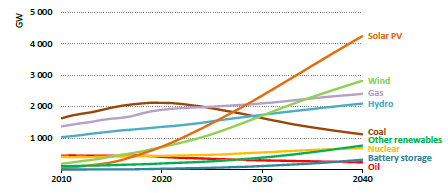
\includegraphics[width=10cm]{GlobalEnergy.PNG}
\caption[Evolution of total generation capacity under Sustainable Development Scenario by IEA]{Evolution of total generation capacity under Sustainable Development Scenario by IEA \cite{WEO}}
\label{Figure:global}
\end{figure}
\newline 
\noindent
In addition to the growing importance of small-scale renewables, a second trend in the electricity market that enhances the effect of utility death spiral is the gradual liberalization of the electricity market, especially in the European Union. The design of the market in its current state allows participants to join into the open market and set up some local DERs generation to fill up a local demand gap. In reality, however, this local DERs adoption is often performed by individuals with little information concerning the market because of the absence of active demand side management and access to real-time information. DERs adoption will, therefore, often be done by actors with limited or imperfect information about the market they are operating in. This imperfect DERs adoption and operation will often impose an additional burden on the utilities and grid operators, since the DERs will cause additional stresses on the grid, making it more challenging for the utility providers to maintain grid balance and stability \cite{EnergyMarket}. 
\newline \newline \noindent
One of the implications of these trends in investments in electricity generation assets is that many more actors will be involved in the investment decision making process, since the nameplate capacity of DERs is lower than that of large generation plants. Whereas historically one central decision maker would choose in what assets to invest, there is a gradual evolution towards a situation where, in theory, every household could make a decision about their means of electricity production and storage. These two opposing scenarios have their implications on the way investment decisions are made. A central decision maker will, most likely, be well informed about all options that can be invested in. In addition, he will likely make decision on a rational basis, since he has dedicated research teams to do so. A household, on the other hand, will be less informed and rational in its investment decisions related to electricity generation assets. In the context of the energy transition and reducing the consumption of fossil fuels of emission of GHG, reducing or transforming the energy consumption on a household level is an important step in the global emission reduction effort \cite{Totalenergy}. Of this total energy consumption, electricity consumption contributes significantly. A good understanding of the investment decisions in electricity related items on a residential level, therefore, is of major importance to be able to make the reduction in overall emissions as efficient as possible. So far, however, this potential has remained underdeveloped \cite{underdeveloped}. In this Thesis, therefore, these investment decisions will be further investigated with a particular focus on the effects  of the DERs adoption on the utility death spiral.
\newline \newline \noindent
The research that has been hitherto conducted in these areas has often had a large amount of assumptions about the actor's behavior that imply rationality, full information and an objective assessment of all facts available. To accurately model the behavior of households or individuals, however, these assumptions must be tweaked. As mentioned earlier, in the current liberalised electricity market, all actors can participate in the supply side of the electricity market, often lacking decent information on the demand, balance and pricing that prevails in the market \cite{EnergyMarket}. Rather than considering the objective value of a few different options to invest in, the crucial parameter in household decision making is the subjective value an actor will attribute to several decision options. These behavioral decision phenomena have been extensively researched in behavioral economic theories like expected utility theory, rank-dependent utility theory and prospect theory. These theories, especially prospect theory, are the basis for the analysis of decision making by individuals or households.  
\newline \newline \noindent
Although these behavioral finance theories are useful in increasing the understanding of decision making by households, the only subjective value (or utility) they consider is an economic one. The decision making of a household in DERs adoption, though, is one that has more motivations than a purely economic one. In the case of individual or household-level decisions, there are social, cultural, environmental and other circumstantial factors that need to be accounted for. In the scope of this Thesis, these additional effects will be represented as the social utility of an investment decision. This will be done through the peer influence, which will consider the influence actors can extert on each other in their decision making \cite{peer}. 
\subsection{Research question and contribution}
The general aim of this research is to determine what the effect is of different policies on DERs adoption and the utility death spiral. These policies include annual net volumetric tariff, annual offtake capacity tariff, net billing and battery subsidies. The main research question of this Thesis, therefore, will be:
\newline\newline
\textbf{Research question 1: What is the effect of annual net metering, annual offtake capacity tariff, net billing and battery subsidies on both households' DERs adoption under uncertainty and the utility death spiral?}
\newline\newline
Since prospect theory is used and interaction between households and the DSO is assumed, there are a some important variables in the system whose sensitivity to the model should be determined. An underlying question in this Thesis, therefore, is to what extent variables like risk aversion, peer influence and variable network charges, among other factors, will shape a household's DERs adoption. The effect of DERs adoption on the revenues of the utilities and distribution grid operators will also be examined. The implementation of prospect theory also gives rise to the thought of what the added value of this theory in this setting is. This objective motivated the following research sub-questions:
\newline\newline
\textbf{Research sub-question 1: What is the effect of risk aversion and network charges on both the DERs adoption on a household level and the utility death spiral?}
\newline \newline
\textbf{Research sub-question 2: What is the added value of using a cumulative prospect theory to model investment decision making, compared to expected utility theory?}
\newline \newline \noindent
These questions will be addressed within a defined scope: the spatial scope is a set of households interacting with each other and a DSO, while the time scope is the lifetime of the technology at hand (being about 20 years). The scope of this research is at the household level because the actors at this level of analysis have access to limited amounts of information and will often behave irrationally in their usage of this information. Thereby, they will take less rational investment decisions. In the development and analysis of this model, it is worth noting two matters. First of all, since this research focuses more on the qualitative insights rather than a quantitative forecast of a certain use case, insights into the different aspects of the model through extensive sensitivity analysis of all parameters are extremely important to gain a comprehensive understanding of the model dynamics. The parameters listed in Research Sub-question 1 (risk aversion, peer influence and network charges) are the most important ones, but other seemingly less influential parameters will also be tested. With these insights, the developed model can be compared with other models as to its results and parameter sensitivity, making Research Sub-question 1 complementary to Research Question 1. In addition, Research Sub-question 2 will address the novelty of CPT in the modeling framework by comparing the results those of the currently used decision making theory, being the EUT. By addressing this main research question and the two research sub-questions, sufficient insights into the model should be obtained to determine in which domains the model can be used for further research.
\subsection{Structure}
This Thesis consists of five chapters. In \textbf{Chapter 2}, the Literature Review, the in the relevant domains will be summarized. Here, the investments in DERs at the household level will be discussed. This will be done by initially focusing on the trends in DERs investments and a discussion of the different emerging DERs technologies, only to elaborate on the investment characteristics and drivers in the following section. Since it also is an important part of this research, the utility death spiral will be discussed separately. In \textbf{Chapter 3}, the Theory and Methods, the concepts and modeling considerations required to describe the DERs adoption will be discussed. This includes the discussion and implementation of the theories and methods that were resorted to in the model development. These include complex adaptive systems theory, prospect theory (and the concepts of behavioral economics like bounded rationality and sub-optimal decision making) and agent-based modeling. In \textbf{Chapter 4}, the Model Design, the theories and methods of Chapter 3 will be used to describe the model. First, the relevance of the chosen modeling techniques in the consumer-centric energy system of this Thesis will be discussed. Subsequently, the model will first be discussed conceptually, after which the model will be described in detail. In \textbf{Chapter 5}, the Results and Discussion, the data resulting from testing different policies in the model will be discussed. In the given framework of the model, this will be done by analyzing how the model results vary as a function of a few key parameters (Network charge, peer influence, loss aversion etc.). Note that the main goal is striving for qualitative insights here rather than quantitative predictions for a specific use case. In \textbf{Chapter 6}, after having discussed the results that the model provides, the key findings of this research as well as the model limitations will be discussed and placed in the broader perspective of the ongoing research.
\newline \newline \noindent
A graphical overview of the structure of this Thesis can be found in Figure \ref{Figure:struct}.
\newline 
\begin{figure}[h!]
\centering
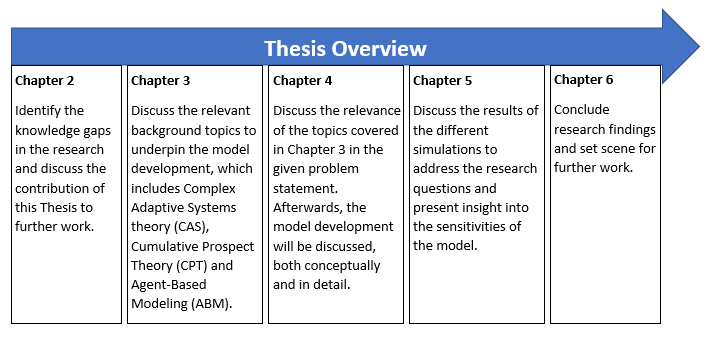
\includegraphics[width=\textwidth]{overview.PNG}
\caption[Overview Thesis]{Overview Thesis}
\label{Figure:struct}
\end{figure}
\newline 
\noindent